\cleardoublepage
\chapter{STUDI LITERATUR}
\label{chap:studi-literatur}

Bab ini menyajikan hasil studi literatur sebagaimana ditetapkan pada Subbab I.5.1. Studi literatur dilakukan untuk membangun fondasi teoritis yang mendasari perancangan dan implementasi sistem \textit{Smart Waste Bin} berbasis IoT. Pembahasan mencakup tiga topik utama: pengelolaan sampah dan tantangannya dalam konteks lingkungan kampus, teknologi \textit{Internet of Things} beserta arsitektur dan komponen yang relevan, serta studi terkait sistem \textit{Smart Waste Bin} yang telah dikembangkan sebelumnya.

% ============================================================
\section{Pengelolaan Sampah}
% ============================================================

Pengelolaan sampah merupakan kegiatan sistematis yang mencakup pengumpulan, pengangkutan, pemrosesan, daur ulang, dan pembuangan material sampah yang dihasilkan dari aktivitas manusia. Pengelolaan sampah yang efektif harus mempertimbangkan aspek teknis, ekonomi, lingkungan, dan sosial untuk mencapai tujuan keberlanjutan \autocite{giurea2024}. Sistem pengelolaan sampah yang baik tidak hanya berfokus pada pembuangan akhir, tetapi juga pada pengurangan volume sampah dari sumbernya, pemilahan, dan pemanfaatan kembali material yang masih memiliki nilai.

\subsection{Konsep Dasar Pengelolaan Sampah}

Dalam konteks hierarki pengelolaan sampah, terdapat beberapa tingkatan prioritas yang harus dipertimbangkan berdasarkan \textit{Waste Framework Directive}. Tingkatan tertinggi adalah pencegahan dan pengurangan sampah di sumber (\textit{waste prevention and reduction}), diikuti oleh persiapan untuk penggunaan kembali (\textit{preparing for reuse}), daur ulang (\textit{recycling}), pemulihan energi (\textit{energy recovery}), dan terakhir adalah pembuangan akhir (\textit{disposal}) \autocite{ec2008}. Pendekatan hierarkis ini menekankan pentingnya upaya preventif dan pemanfaatan nilai ekonomi dari sampah sebelum melakukan pembuangan.

Pengelolaan sampah modern juga menerapkan prinsip \textit{circular economy} yang bertujuan untuk meminimalkan limbah dan memaksimalkan pemanfaatan sumber daya melalui sistem yang tertutup. \textit{Circular economy} didefinisikan sebagai sistem regeneratif di mana \textit{input} sumber daya, limbah, emisi, dan kebocoran energi diminimalkan melalui strategi memperlambat, menutup, dan mempersempit aliran material dan energi \autocite{geissdoerfer2017}. Dalam konteks institusi pendidikan tinggi, penerapan \textit{circular economy} mencakup tiga dimensi keberlanjutan: ekonomi, ekologi, dan sosial, yang bekerja secara sinergis untuk menciptakan sistem pengelolaan sampah yang tidak hanya ramah lingkungan, tetapi juga bertanggung jawab secara ekonomi dan sosial \autocite{giurea2024}.

\textit{Sustainable Development Goals} (SDGs) yang ditetapkan oleh \textit{United Nations} juga menekankan pentingnya pengelolaan sampah berkelanjutan sebagai bagian dari upaya mencapai dunia yang lebih berkelanjutan dan berkeadilan pada tahun 2030 \autocite{un2015}. Pengelolaan sampah yang efektif berkontribusi pada beberapa SDGs, termasuk kota dan komunitas berkelanjutan (SDG 11), konsumsi dan produksi yang bertanggung jawab (SDG 12), serta aksi iklim (SDG 13).

\subsection{Tantangan Pengelolaan Sampah pada Lingkungan Kampus}

Lingkungan kampus dan gedung perkuliahan memiliki karakteristik unik dalam hal pengelolaan sampah yang membedakannya dari lingkungan perkotaan pada umumnya. Institusi pendidikan tinggi menghadapi tantangan khusus karena kepadatan populasi yang tinggi, variasi aktivitas yang beragam, dan pola penggunaan yang dinamis sepanjang hari dan minggu \autocite{bahcelioglu2020}. Karakteristik ini menyebabkan volume dan komposisi sampah yang dihasilkan sangat bervariasi tergantung pada waktu, aktivitas akademik, dan kegiatan yang berlangsung di gedung.

Berdasarkan \textit{review} komprehensif terhadap penelitian tentang pengelolaan sampah di institusi pendidikan tinggi, rata-rata tingkat produksi sampah adalah $0{,}19 \pm 0{,}21$ kg/hari per orang (median $0{,}093$ kg/hari per orang) \autocite{rodriguez2024}. Komposisi sampah didominasi oleh sampah organik yang mencapai rata-rata $30 \pm 19$\% dari total sampah, diikuti oleh kertas dan kardus ($23 \pm 13$\%), dan plastik ($18 \pm 11$\%) \autocite{bahcelioglu2020}.

Salah satu tantangan utama adalah keterbatasan data mengenai pola pembuangan sampah. Penelitian menunjukkan bahwa sebagian besar institusi pendidikan mengalami kesulitan dalam melacak kapan, di mana, dan berapa banyak sampah yang dihasilkan karena tidak memiliki sistem \textit{monitoring} yang memadai \autocite{bahcelioglu2020}. Tanpa data yang \textit{reliable}, pengambilan keputusan terkait pengelolaan sampah menjadi tidak akurat, menghambat perencanaan strategis yang efektif, dan mempersulit pelacakan \textit{progress} terhadap tujuan pengurangan sampah \autocite{sensoneo2024}.

Tantangan lain yang dihadapi adalah variasi temporal dalam produksi sampah. Kampus dapat mengalami fluktuasi volume sampah yang signifikan antara periode aktif perkuliahan dan periode libur, dengan volume sampah dapat turun hingga sebagian kecil dari volume normal dalam waktu singkat \autocite{roadrunner2024}. Pola pembuangan sampah juga sangat dipengaruhi oleh jadwal perkuliahan, waktu istirahat, dan aktivitas khusus seperti seminar atau acara. Tanpa pemahaman yang baik terhadap pola temporal ini, alokasi sumber daya untuk pengumpulan sampah menjadi tidak efisien.

Tingkat partisipasi pengguna dalam pemilahan sampah juga menjadi tantangan tersendiri. Meskipun banyak kampus telah menyediakan fasilitas untuk pemilahan sampah, tingkat kepatuhan dan konsistensi dalam pemilahan masih rendah. Kontaminasi dalam aliran daur ulang terjadi ketika material yang tidak dapat didaur ulang tercampur dengan yang dapat didaur ulang, mengurangi efisiensi program daur ulang dan meningkatkan biaya pemrosesan \autocite{sensoneo2024}.

Tantangan operasional lainnya mencakup pengumpulan sampah yang tidak efisien, dengan \textit{pickup} yang sering dilakukan pada tempat sampah yang masih kosong atau sebagian terisi, mengakibatkan pemborosan bahan bakar, jam kerja, dan biaya pemeliharaan. Kondisi \textit{bin} yang meluap tidak hanya menciptakan lingkungan kampus yang tidak menarik, tetapi juga berkontribusi pada kontaminasi aliran daur ulang karena orang berhenti memilah sampah dan membuangnya ke \textit{bin} kosong terdekat tanpa memperhatikan jenis \textit{bin} tersebut \autocite{sensoneo2024}.

\subsection{Data dalam Pengelolaan Sampah}

Data merupakan fondasi penting dalam pengambilan keputusan untuk pengelolaan sampah yang efektif dan efisien. Sistem pengelolaan sampah berbasis data memungkinkan identifikasi pola, prediksi kebutuhan, dan optimalisasi operasional yang tidak dapat dicapai melalui pendekatan konvensional. Dengan data yang akurat dan terstruktur, pengelola dapat memahami karakteristik sampah yang dihasilkan, mengidentifikasi area atau waktu yang memerlukan perhatian khusus, dan merancang strategi pengelolaan yang lebih responsif.

Keputusan yang diambil berdasarkan data sampah yang tidak \textit{reliable} dapat mengganggu akurasi pelaporan keberlanjutan dan menghambat perencanaan strategis yang efektif. Tanpa data yang dapat diandalkan, sulit untuk melacak kemajuan terhadap tujuan pengurangan sampah, mengidentifikasi inefisiensi, atau mengoptimalkan jadwal pengumpulan \autocite{sensoneo2024}.

Pemanfaatan teknologi sensor ultrasonik, \textit{Time-of-Flight} (ToF), dan perangkat IoT lainnya memungkinkan \textit{monitoring} \textit{bin} secara \textit{real-time}, yang dapat memberikan \textit{alert} ketika \textit{bin} mendekati atau mencapai kapasitas penuh \autocite{pires2025}. Sistem ini tidak hanya meningkatkan efisiensi operasional, tetapi juga mencegah kondisi \textit{bin} yang meluap yang dapat menciptakan risiko kesehatan dan lingkungan.

Selain itu, data pembuangan sampah dapat memberikan \textit{insight} berharga untuk pengembangan program edukasi dan perubahan perilaku. Dengan memahami kapan dan di mana sampah paling banyak dihasilkan, serta jenis sampah yang dominan, institusi dapat merancang intervensi yang lebih spesifik untuk mengurangi produksi sampah atau meningkatkan tingkat daur ulang. Dalam konteks institusi pendidikan tinggi, data pengelolaan sampah juga berkontribusi pada pelaporan keberlanjutan (\textit{sustainability reporting}) yang semakin menjadi standar dalam akreditasi dan \textit{ranking} universitas internasional \autocite{bahcelioglu2020}.

% ============================================================
\section{\textit{Internet of Things}}
% ============================================================

\textit{Internet of Things} (IoT) didefinisikan sebagai konsep yang menghubungkan benda fisik dan virtual melalui jaringan internet untuk memungkinkan pertukaran data secara otomatis. Kevin Ashton, yang pertama kali memperkenalkan istilah IoT pada tahun 1999, menjelaskan bahwa IoT memungkinkan komputer untuk secara mandiri mengumpulkan informasi tanpa bantuan manusia, sehingga dapat mengurangi pemborosan, biaya, serta meningkatkan efisiensi \autocite{ashton2009}.

IoT dapat dipahami sebagai keberadaan pervasif dari berbagai objek yang mampu berinteraksi dan bekerja sama satu sama lain melalui skema pengalamatan yang unik untuk mencapai tujuan bersama \autocite{atzori2010}. \textit{International Telecommunication Union} (ITU-T) mendefinisikan IoT sebagai infrastruktur global yang mendukung layanan canggih melalui konektivitas benda fisik dan virtual menggunakan teknologi informasi dan komunikasi yang terus berkembang \autocite{itu2012}. Sementara itu, IoT \textit{European Research Cluster} (IERC) mendefinisikan IoT sebagai infrastruktur jaringan global yang dinamis dengan kemampuan konfigurasi mandiri, menggunakan protokol komunikasi standar dan interoperabel \autocite{iotec2014}.

Dengan berbagai definisi tersebut, IoT secara umum dapat dipahami sebagai infrastruktur global yang menghubungkan benda fisik dan virtual melalui jaringan internet, memungkinkan pertukaran data secara otomatis tanpa intervensi manusia yang signifikan. IoT memberikan manfaat signifikan dalam berbagai sektor seperti transportasi, kesehatan, manufaktur, dan kota pintar.

\subsection{Arsitektur \textit{Internet of Things}}

Arsitektur IoT bertujuan untuk menciptakan sinergi antara berbagai sistem yang memungkinkan perangkat-perangkat IoT untuk berkomunikasi dan saling beroperasi secara otomatis. Salah satu model arsitektur IoT yang paling fundamental dan banyak diadopsi adalah model tiga \textit{layer} yang terdiri dari \textit{Perception Layer}, \textit{Network Layer}, dan \textit{Application Layer} \autocite{sethi2017}. Model ini menyediakan kerangka dasar untuk memahami bagaimana komponen-komponen IoT berinteraksi dari tingkat perangkat fisik hingga aplikasi pengguna akhir.

\begin{figure}[H]
  \caption{IoT Reference Model 3 \textit{Layer} \autocite{sethi2017}}
  \label{fig:iot-3layer}
  \centering
  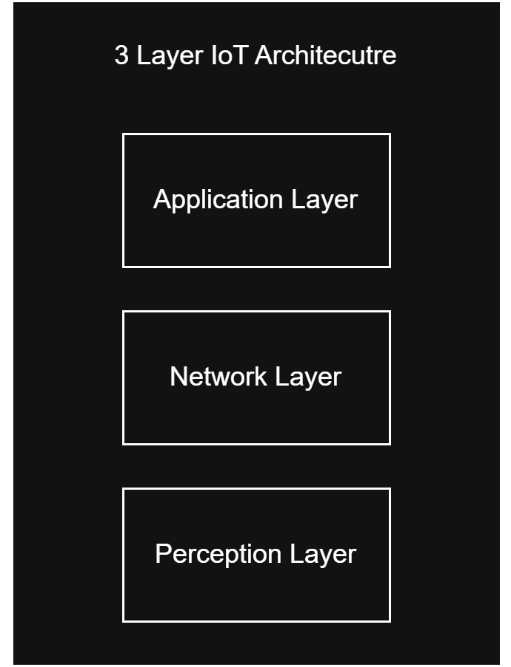
\includegraphics[width=0.5\textwidth]{images/iot-3layer.png}
  % RENAME: image5.png → iot-3layer.png di folder images/
\end{figure}

Berikut adalah penjelasan untuk setiap \textit{layer} pada arsitektur IoT berdasarkan Gambar \ref{fig:iot-3layer}:

\begin{enumerate}
  \item \textit{Perception Layer}

  \textit{Perception Layer}, yang juga dikenal sebagai \textit{Physical Layer} atau \textit{Device Layer}, merupakan lapisan paling bawah dalam arsitektur IoT. \textit{Layer} ini terdiri dari perangkat fisik seperti sensor, aktuator, \textit{RFID tags}, dan perangkat IoT lainnya yang berinteraksi langsung dengan lingkungan fisik \autocite{alfuqaha2015}. Fungsi utamanya adalah mengumpulkan data dari lingkungan sekitar, seperti suhu, kelembaban, tekanan, gerak, atau parameter lainnya sesuai dengan jenis sensor yang digunakan.

  Dalam konteks sistem \textit{Smart Waste Bin}, \textit{Perception Layer} mencakup sensor ultrasonik atau sensor \textit{Time-of-Flight} yang dipasang pada tempat sampah untuk mengukur tingkat kepenuhan secara periodik. Karakteristik penting dari \textit{layer} ini adalah kemampuannya untuk beroperasi dalam berbagai kondisi lingkungan, efisiensi energi untuk perangkat berbasis baterai, dan akurasi dalam pengukuran.

  \item \textit{Network Layer}

  \textit{Network Layer} berfungsi sebagai jembatan komunikasi yang menghubungkan \textit{Perception Layer} dengan \textit{Application Layer}. \textit{Layer} ini bertanggung jawab untuk transmisi data yang dikumpulkan oleh sensor ke sistem pemrosesan atau \textit{cloud server} \autocite{alfuqaha2015}. \textit{Network Layer} menggunakan berbagai protokol komunikasi dan teknologi jaringan seperti Wi-Fi, Ethernet, LoRaWAN, NB-IoT, Zigbee, Bluetooth, atau protokol lainnya tergantung pada kebutuhan jarak, \textit{bandwidth}, dan konsumsi energi.

  Dalam sistem \textit{Smart Waste Bin}, \textit{Network Layer} dapat menggunakan koneksi Wi-Fi atau \textit{cellular network} (seperti 4G/5G) untuk mengirimkan data tingkat kepenuhan sampah dari lokasi tempat sampah ke \textit{server} pusat secara periodik.

  \item \textit{Application Layer}

  \textit{Application Layer} merupakan lapisan tertinggi dalam arsitektur IoT yang berfungsi untuk menyediakan layanan dan antarmuka kepada pengguna akhir \autocite{alfuqaha2015}. \textit{Layer} ini mencakup aplikasi yang memproses, menganalisis, dan memvisualisasikan data yang diterima dari \textit{Network Layer}. Pada \textit{layer} ini terdapat sistem manajemen data, analitik, dan \textit{dashboard} yang memungkinkan pengguna untuk memantau kondisi, mengambil keputusan, atau melakukan kontrol terhadap perangkat IoT.

  Dalam konteks sistem \textit{Smart Waste Bin}, \textit{Application Layer} mencakup sistem \textit{database} untuk menyimpan data pembuangan sampah secara terstruktur, serta \textit{dashboard} yang memungkinkan pengelola untuk melihat status tempat sampah dan hasil analisis pola pembuangan.
\end{enumerate}

\subsection{Komponen Perangkat Keras pada IoT}

Implementasi sistem IoT memerlukan komponen \textit{hardware} yang berfungsi sebagai jembatan antara dunia fisik dan dunia digital. Komponen-komponen ini berada pada \textit{Perception Layer} dalam arsitektur IoT dan berperan dalam pengumpulan data dari lingkungan serta pemrosesan awal sebelum data dikirimkan ke sistem \textit{backend}.

\begin{enumerate}
  \item \textit{Microcontroller}

  \textit{Microcontroller} merupakan komputer kecil dalam satu \textit{chip} yang berfungsi sebagai ``otak'' dari perangkat IoT. \textit{Microcontroller} bertanggung jawab untuk membaca data dari sensor, memproses data tersebut, dan mengirimkannya ke \textit{server} atau \textit{cloud} melalui protokol komunikasi tertentu. Berbeda dengan mikroprosesor yang memerlukan komponen eksternal, \textit{microcontroller} mengintegrasikan semua komponen dalam satu \textit{chip}, termasuk \textit{CPU}, \textit{RAM}, \textit{ROM/Flash memory}, dan berbagai \textit{peripheral}.

  Tabel \ref{tab:perbandingan-mcu} menyajikan perbandingan empat \textit{platform microcontroller} yang umum digunakan dalam aplikasi IoT.

  \begin{table}[H]
    \caption{Perbandingan Arduino, Raspberry Pi, ESP8266 NodeMCU, dan ESP32 \autocite{ooko2019, espressif2021}}
    \label{tab:perbandingan-mcu}
    \begin{tabularx}{\textwidth}{| l | X | X | X | X |}
      \hline
      \textbf{Kriteria} & \textbf{Arduino} & \textbf{Raspberry Pi} & \textbf{ESP8266 NodeMCU} & \textbf{ESP32} \\
      \hline
      Pengembang & Arduino & Raspberry Pi Foundation & ESP8266 Open Source Community & Espressif Systems \\
      \hline
      Tipe & Single Board \textit{Microcontroller} & Mini Computer & Single Board \textit{Microcontroller} & Single Board \textit{Microcontroller} \\
      \hline
      Sistem Operasi & None & Linux & XTOS & FreeRTOS \\
      \hline
      CPU & Atmel, ARM & ARM Cortex & LXT106 & Dual-Core Xtensa 32-bit LX6 \\
      \hline
      Kecepatan \textit{Clock} & 16 MHz & 1,2 GHz & 26--52 MHz & 160--240 MHz \\
      \hline
      Memori & 32 KB & 1--4 GB & Hingga 128 MB & 520 KB SRAM \\
      \hline
      Penyimpanan & 1 KB & MicroSDHC & 4 MB \textit{Flash} & Hingga 16 MB \textit{Flash} \\
      \hline
      Tegangan Operasi & 5V & 5V & 3,3V & 3,3V \\
      \hline
      Konektivitas & I/O & SPI, I2C, UART, GPIO & UART, GPIO & UART, GPIO, Wi-Fi, BLE, SPI, I2C \\
      \hline
    \end{tabularx}
  \end{table}

  Arduino merupakan \textit{microcontroller} sederhana yang ideal untuk pengendalian perangkat keras dasar dengan kebutuhan komputasi ringan. ESP8266 NodeMCU dirancang khusus untuk aplikasi IoT yang memerlukan konektivitas jaringan dengan biaya rendah melalui Wi-Fi terintegrasi. ESP32 merupakan evolusi dari ESP8266 yang menawarkan peningkatan signifikan dalam hal performa, dilengkapi dengan prosesor \textit{dual-core} Xtensa 32-bit LX6 berkecepatan hingga 240 MHz, konektivitas Wi-Fi dan \textit{Bluetooth Low Energy} (BLE) secara simultan, serta dukungan sistem operasi FreeRTOS untuk pengelolaan \textit{multitasking} \autocite{espressif2021}. Raspberry Pi memiliki karakteristik yang lebih menyerupai komputer mini lengkap, cocok untuk aplikasi yang memerlukan pemrosesan data kompleks atau \textit{interfacing} dengan berbagai \textit{peripheral}, meskipun dengan konsumsi daya yang lebih tinggi.

  \item Sensor dan \textit{Actuator}

  Sensor adalah perangkat yang mendeteksi dan merespons \textit{input} dari lingkungan fisik, mengubah fenomena fisik seperti suhu, kelembaban, tekanan, cahaya, atau gerakan menjadi sinyal elektrik yang dapat diproses oleh \textit{microcontroller}. Sensor dapat dikategorikan sebagai sensor aktif yang memerlukan sumber daya eksternal, dan sensor pasif yang menghasilkan \textit{output} tanpa sumber daya eksternal. Dalam konteks IoT, sensor juga dikategorikan berdasarkan jenis data yang dihasilkan: sensor analog yang menghasilkan sinyal kontinu, dan sensor digital yang menghasilkan sinyal diskrit.

  \textit{Actuator}, di sisi lain, adalah perangkat yang melakukan aksi fisik berdasarkan perintah dari sistem kontrol, mengubah sinyal elektrik menjadi gerakan mekanis, panas, cahaya, atau bentuk energi lainnya. Dalam sistem IoT, \textit{actuator} memungkinkan sistem untuk tidak hanya mengamati lingkungan tetapi juga berinteraksi dan mengubah kondisi lingkungan berdasarkan data yang dikumpulkan.
\end{enumerate}

\subsection{Protokol Komunikasi IoT}

Protokol komunikasi dalam sistem IoT memainkan peran krusial dalam memastikan interoperabilitas dan efisiensi pertukaran data antar perangkat yang terhubung. Protokol-protokol ini dirancang untuk mengatasi tantangan spesifik yang dihadapi oleh perangkat IoT, seperti keterbatasan daya, \textit{bandwidth} terbatas, dan kebutuhan akan komunikasi yang andal dalam berbagai kondisi jaringan \autocite{alfuqaha2015}.

\begin{enumerate}
  \item HTTP/HTTPS (\textit{Hypertext Transfer Protocol})

  HTTP merupakan protokol komunikasi berbasis \textit{request-response} yang beroperasi di atas TCP (\textit{Transmission Control Protocol}). HTTPS adalah versi aman dari HTTP yang menggunakan enkripsi SSL/TLS untuk melindungi data selama transmisi. Kelebihan HTTP/HTTPS meliputi kompatibilitas yang luas dengan infrastruktur web yang ada dan kemudahan integrasi dengan layanan \textit{cloud}. Namun, HTTP memiliki \textit{overhead} yang relatif besar dibandingkan protokol IoT lainnya \autocite{alfuqaha2015}.

  \item MQTT (\textit{Message Queuing Telemetry Transport})

  MQTT adalah protokol \textit{messaging} berbasis \textit{publish-subscribe} yang dirancang khusus untuk perangkat dengan sumber daya terbatas dan jaringan dengan \textit{bandwidth} rendah atau tidak stabil. Protokol ini beroperasi di atas TCP dan menggunakan model \textit{broker} sentral yang mengelola komunikasi antara \textit{publisher} (perangkat yang mengirim data) dan \textit{subscriber} (aplikasi yang menerima data).

  Arsitektur \textit{publish-subscribe} MQTT memberikan beberapa keunggulan: \textit{decoupling} antara \textit{publisher} dan \textit{subscriber} yang memungkinkan skalabilitas lebih baik, dukungan tiga tingkat \textit{Quality of Service} (QoS 0, 1, dan 2), serta \textit{overhead} protokol yang sangat kecil dengan \textit{header} minimum hanya 2 \textit{bytes}. MQTT juga mendukung fitur \textit{retained messages} dan \textit{last will and testament} (LWT) yang menjadikannya sangat populer dalam aplikasi \textit{monitoring} dan telemetri IoT \autocite{alfuqaha2015}.

  \item CoAP (\textit{Constrained Application Protocol})

  CoAP adalah protokol aplikasi web yang dirancang khusus untuk perangkat terkendali (\textit{constrained devices}) dengan memori, daya pemrosesan, dan \textit{bandwidth} yang sangat terbatas. Berbeda dengan HTTP yang menggunakan TCP, CoAP beroperasi di atas UDP (\textit{User Datagram Protocol}), yang mengurangi \textit{overhead} komunikasi. CoAP cocok untuk aplikasi IoT yang memerlukan komunikasi \textit{RESTful} namun beroperasi pada perangkat dengan keterbatasan sumber daya yang signifikan \autocite{alfuqaha2015}.
\end{enumerate}

Pemilihan protokol komunikasi bergantung pada karakteristik perangkat, kebutuhan aplikasi, dan kondisi jaringan. HTTP/HTTPS cocok untuk sistem yang memerlukan integrasi mudah dengan infrastruktur web. MQTT ideal untuk aplikasi yang memerlukan komunikasi asinkron dengan \textit{overhead} rendah. CoAP merupakan pilihan terbaik untuk perangkat dengan keterbatasan sumber daya yang ekstrem.

% ============================================================
\section{Node-RED}
% ============================================================

Node-RED adalah \textit{platform} pemrograman visual berbasis aliran (\textit{flow-based}) yang dikembangkan oleh IBM dan kini merupakan proyek \textit{open-source} di bawah naungan OpenJS Foundation. \textit{Platform} ini dirancang untuk menghubungkan perangkat keras, API, dan layanan daring dengan cara yang mudah dipahami melalui antarmuka berbasis \textit{browser}. Node-RED berjalan di atas \textit{runtime} Node.js dan memungkinkan pengguna untuk membuat alur pemrosesan data dengan cara menyusun dan menghubungkan \textit{node}-\textit{node} fungsional tanpa harus menulis kode secara eksplisit \autocite{openjs2024}.

Konsep utama Node-RED adalah \textit{flow}, yaitu rangkaian \textit{node} yang saling terhubung melalui kabel (\textit{wire}). Terdapat tiga kategori \textit{node} utama: \textit{input node} sebagai sumber data (misalnya MQTT In, HTTP In), \textit{processing node} yang memanipulasi data (misalnya \textit{Function}, \textit{Switch}, \textit{Change}), serta \textit{output node} yang mengirimkan data ke tujuan akhir. Arsitektur ini menjadikan Node-RED sangat fleksibel sebagai komponen \textit{middleware} dalam ekosistem IoT, karena mampu menjembatani protokol komunikasi yang berbeda-beda \autocite{blackstock2016}.

Dalam konteks sistem IoT, Node-RED sering digunakan sebagai lapisan \textit{middleware} yang menerima data dari perangkat sensor melalui protokol MQTT atau HTTP, kemudian memvalidasi, mentransformasi, dan meneruskan data tersebut ke sistem penyimpanan atau layanan lainnya. Keunggulan Node-RED meliputi kemudahan konfigurasi melalui antarmuka visual, ekosistem \textit{node} yang kaya (tersedia lebih dari 4.000 \textit{node} tambahan di repositori publik), serta kemampuan \textit{deployment} yang cepat tanpa memerlukan proses kompilasi \autocite{clerissi2018}.

% ============================================================
\section{Studi Terkait}
% ============================================================

Bagian ini mengkaji penelitian-penelitian terdahulu yang relevan dengan topik pengembangan sistem \textit{Smart Waste Bin}, dengan fokus pada metode yang digunakan, hasil yang diperoleh, dan \textit{gap} yang menjadi dasar penelitian ini.

\subsection{Sistem \textit{Smart Waste Bin} Berbasis IoT}

\textcite{latifah2021} mengembangkan sistem \textit{Automated Trash Volume Monitoring} berbasis IoT untuk meningkatkan efisiensi pengelolaan sampah perkotaan. Sistem yang dikembangkan mengintegrasikan sensor ultrasonik HC-SR04 untuk \textit{monitoring} tingkat kepenuhan tempat sampah secara \textit{real-time}, mikrokontroler NodeMCU ESP8266 sebagai unit pemrosesan, dan \textit{platform} Blynk sebagai \textit{interface} untuk visualisasi dan notifikasi kepada petugas kebersihan. Sistem juga dilengkapi dengan servo motor yang mengoperasikan mekanisme pembukaan dan penutupan tutup tempat sampah secara otomatis ketika sensor infrared mendeteksi keberadaan pengguna pada jarak 50 cm.

Hasil pengujian sistem menunjukkan akurasi pengukuran volume sebesar 97\% dengan \textit{margin of error} 3\%, menunjukkan reliabilitas tinggi dalam \textit{monitoring} kondisi tempat sampah. Sistem berhasil mengirimkan notifikasi secara konsisten ketika \textit{threshold} tercapai, dengan \textit{average response time} kurang dari 5 detik dari deteksi hingga notifikasi diterima. Penelitian ini berkontribusi dalam demonstrasi \textit{feasibility} sistem IoT untuk \textit{waste management} dengan biaya implementasi yang relatif terjangkau.

\textcite{pires2025} mengembangkan sistem \textit{monitoring} urban berbasis IoT menggunakan teknologi sensor \textit{Time-of-Flight} (ToF) untuk pemantauan tingkat kepenuhan tempat sampah secara \textit{real-time}. Penelitian ini menggunakan sensor VL53L0X yang dipasang pada tempat sampah untuk mengukur jarak ke permukaan sampah dengan presisi tinggi, dikombinasikan dengan mikrokontroler yang dilengkapi konektivitas jaringan untuk transmisi data ke \textit{platform} pusat. Keunggulan utama pendekatan ini dibandingkan sensor ultrasonik konvensional adalah akurasi pengukuran yang lebih tinggi pada berbagai kondisi permukaan dan jenis material sampah.

Hasil penelitian menunjukkan bahwa sistem berbasis sensor ToF mampu memberikan akurasi pengukuran yang lebih konsisten dibandingkan sensor ultrasonik dalam kondisi penggunaan nyata. Data yang dikumpulkan selama periode evaluasi menunjukkan pola temporal yang jelas dalam pembuangan sampah, dengan \textit{peak} aktivitas yang berulang pada waktu-waktu tertentu. Penelitian ini memperkuat argumen bahwa sistem IoT berbasis data dapat menghasilkan \textit{insight} yang bernilai untuk optimalisasi pengelolaan sampah perkotaan.

Dibandingkan dengan kedua penelitian tersebut, penelitian ini memiliki perbedaan yang signifikan. Pertama, fokus utama bukan hanya pada \textit{monitoring} kepenuhan, tetapi pada analisis pola pembuangan sampah secara temporal untuk menghasilkan \textit{insight} yang dapat digunakan dalam pengambilan keputusan. Kedua, penelitian ini dilakukan pada lingkungan kampus dengan karakteristik yang berbeda dari lingkungan perkotaan umum, dan melibatkan optimasi \textit{firmware} perangkat pihak ketiga untuk menyesuaikan dengan kebutuhan lingkungan kampus. Ketiga, penelitian ini menggunakan arsitektur IoT 4-\textit{layer} yang lebih komprehensif dengan integrasi \textit{middleware} Node-RED, \textit{database} Supabase, dan \textit{dashboard} berbasis Next.js.